\section{Background}
\label{sec:background}

\subsection{Block Floating Point}
Low-precision integer quantization reduces storage and arithmetic cost, but a single tensor-level scaling factor can be dominated by rare large-magnitude values.
This issue is particularly severe in LLM activations, where a small number of outliers may compress most nonoutlier values into a limited set of quantization levels and degrade low-bit accuracy~\cite{smoothquant2023,olive2023,gobo2020}.

Block Floating Point (BFP) provides a more fine-grained accuracy--cost tradeoff by partitioning tensors into fixed-size blocks and assigning an independent shared exponent to each block.
Each element stores only a sign and a low-bit mantissa (Fig.~\ref{fig:data_format}(a)), while the exponent overhead is amortized across the block.
Intra-block computation requires only fixed-point multiply--accumulate operations, enabling BFP to achieve higher accuracy at a cost comparable to integer quantization~\cite{msfp2020,fast2022}.

\begin{figure*}[t]
    \centering
    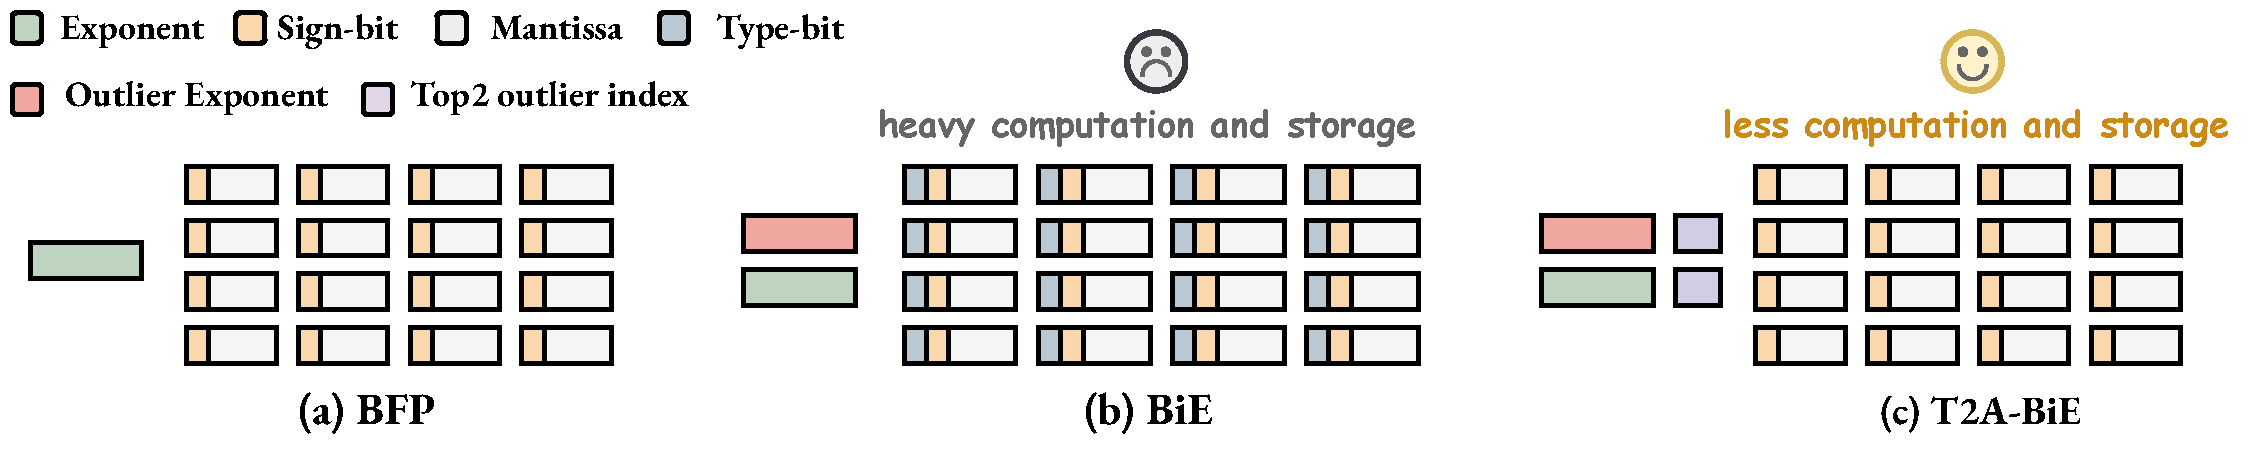
\includegraphics[width=0.95\textwidth]{figures/data-format.pdf}
    \caption{Block-level data formats. (a) Conventional BFP with one shared exponent per block. (b) Bi-exponent BFP (BiE), which adds an outlier exponent and spends a type bit on every element. (c) The proposed Top-2 Activation-only Bi-Exponent BFP (T2A-BiE), which keeps both exponents but replaces the per-element type bits with two outlier indices, so the storage and MAC overhead is lower than that of BiE; weights remain single-exponent BFP as in (a).}
    \label{fig:data_format}
\end{figure*}

\subsection{Deployment Challenges}
Applying BFP to LLM inference acceleration introduces two major bottlenecks.

\textbf{(1) Inter-block floating-point accumulation.}
A state-of-the-art BFP processing element (BFP-PE) can perform MAC operations within each block using low-bit fixed-point arithmetic.
However, shared exponents differ across blocks, so partial sums cannot be directly accumulated in the integer domain.
An FP accumulator (FP-Acc) is therefore required to perform inter-block exponent alignment and floating-point accumulation.
The FP-Acc typically includes alignment, normalization, addition, and fixed-point-to-floating-point conversion logic.
In synthesized low-bit BFP-PE configurations, the FP-Acc accounts for up to 68\% of PE power and 42\% of its area when the PE is driven by LLaMA2-7B's real activation distribution (Fig.~\ref{fig:bfp_pe_ppa}), making it a primary obstacle to improving the energy and area efficiency of BFP accelerators~\cite{bucketgetter2023,winacc2025,smartblock2025}.

\begin{figure}[t]
    \centering
    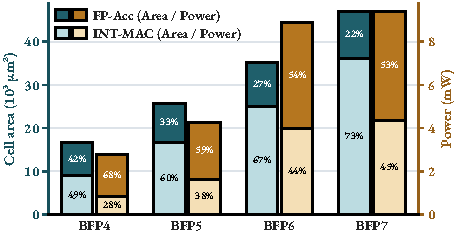
\includegraphics[width=\linewidth]{figures/baseline_bfp_pe_component_power_area.pdf}
    \caption{Component-level power and area of a synthesized baseline BFP-PE. Power is measured under LLaMA2-7B's real activation distribution.}
    \label{fig:bfp_pe_ppa}
\end{figure}

\textbf{(2) Activation outliers.}
BFP confines the influence of an outlier to its local block but does not eliminate the outlier itself.
When a block contains a large-magnitude outlier, the shared exponent is determined by that value, and nonoutlier values in the same block lose a substantial number of effective mantissa bits~\cite{bie2024,oiso2026,bbal2025,harmonia2026}.
This loss becomes more severe as the mantissa width decreases (Fig.~\ref{fig:vanilla_bfp_delta_ppl}).

\begin{figure}[t]
    \centering
    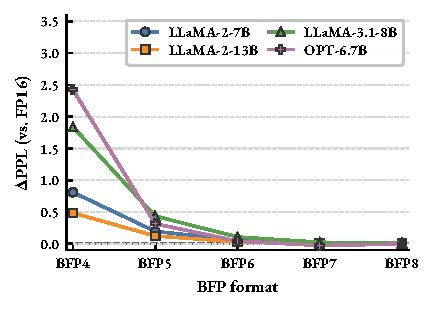
\includegraphics[width=0.9\linewidth]{figures/vanilla_bfp_delta_ppl_g16.pdf}
    \caption{WikiText-2 $\Delta$PPL of vanilla BFP versus FP16 as the mantissa width decreases (group size 16).}
    \label{fig:vanilla_bfp_delta_ppl}
\end{figure}

These two bottlenecks are coupled.
Outliers degrade the precision of nonoutlier values during quantization and can also widen the exponent distribution of resulting partial sums, increasing the likelihood that inter-block updates require the FP-Acc.
Consequently, effective outlier handling has the potential to improve numerical fidelity while simultaneously reducing FP-Acc activity.
This observation motivates the approach developed in this work.

\subsection{Bi-Exponent BFP for Outlier Separation}
\label{subsec:bie}
A common remedy for the precision loss described above is to give outliers their own exponent instead of forcing an entire block to share one.
BiE~\cite{bie2024} and Oiso~\cite{oiso2026} store two shared exponents per block (BiE format), one for nonoutlier values and one for outliers, and prepend a type bit to each element that selects which exponent applies (Fig.~\ref{fig:data_format}(b)).
Nonoutlier values therefore keep their effective mantissa bits even when the block contains a large-magnitude value.

The accuracy gain, however, comes with non-trivial overhead.
Because outliers are inherently rare, a per-element type bit spends storage on every element to describe a small minority, and the two exponents must be applied to both operands of a MAC, yielding four exponent-pair cases that the datapath has to support.
This overhead is what makes a direct combination of bi-exponent BFP with a low-cost accumulator unattractive, and it is the starting point for the format we propose in Section~\ref{sec:design} (Fig.~\ref{fig:data_format}(c)).
